\documentclass[10pt,a4paper]{article}



%%Imports
\usepackage{amsmath}
\usepackage[utf8]{inputenc} % Codificación de entrada
\usepackage[spanish]{babel} % Idioma español
\usepackage[left=2cm,top=2.5cm,right=2cm,bottom=2.5cm]{geometry} % Márgenes
\usepackage{graphicx} % Para incluir imágenes
\usepackage{caption} % Para personalizar los títulos de las figuras
\usepackage{graphicx, float,hyperref,multirow,parskip,xcolor,blindtext,multicol,siunitx}
\usepackage{subcaption} % Para subfiguras
\usepackage{hyperref} % Para hipervínculos
\usepackage[backend=biber,style=numeric,sorting=none]{biblatex} % Para gestionar las referencias bibliográficas
\addbibresource{Referencias.bib} % Archivo .bib con las referencias


\usepackage[spanish,activeacute,es-tabla]{babel}
\usepackage[utf8]{inputenc}
\usepackage{ifthen}
\usepackage{listings}
\usepackage{dsfont}
\usepackage{subcaption}
\usepackage{amsmath}
\usepackage[strict]{changepage}
\usepackage[top=1cm,bottom=2cm,left=1cm,right=1cm]{geometry}%
\usepackage{color}%
\newcommand{\tocarEspacios}{%
	\addtolength{\leftskip}{3em}%
	\setlength{\parindent}{0em}%
}

% Especificacion de procs

\newcommand{\In}{\textsf{in }}
\newcommand{\Out}{\textsf{out }}
\newcommand{\Inout}{\textsf{inout }}

\newcommand{\encabezadoDeProc}[4]{%
	% Ponemos la palabrita problema en tt
	%  \noindent%
	{\normalfont\bfseries\ttfamily proc}%
	% Ponemos el nombre del problema
	\ %
	{\normalfont\ttfamily #2}%
	\
	% Ponemos los parametros
	(#3)%
	\ifthenelse{\equal{#4}{}}{}{%
		% Por ultimo, va el tipo del resultado
		\ : #4}
}

\newenvironment{proc}[4][res]{%
	
	% El parametro 1 (opcional) es el nombre del resultado
	% El parametro 2 es el nombre del problema
	% El parametro 3 son los parametros
	% El parametro 4 es el tipo del resultado
	% Preambulo del ambiente problema
	% Tenemos que definir los comandos requiere, asegura, modifica y aux
	\newcommand{\requiere}[2][]{%
		{\normalfont\bfseries\ttfamily requiere}%
		\ifthenelse{\equal{##1}{}}{}{\ {\normalfont\ttfamily ##1} :}\ %
		\{\ensuremath{##2}\}%
		{\normalfont\bfseries\,\par}%
	}
	\newcommand{\asegura}[2][]{%
		{\normalfont\bfseries\ttfamily asegura}%
		\ifthenelse{\equal{##1}{}}{}{\ {\normalfont\ttfamily ##1} :}\
		\{\ensuremath{##2}\}%
		{\normalfont\bfseries\,\par}%
	}
	\renewcommand{\aux}[4]{%
		{\normalfont\bfseries\ttfamily aux\ }%
		{\normalfont\ttfamily ##1}%
		\ifthenelse{\equal{##2}{}}{}{\ (##2)}\ : ##3\, = \ensuremath{##4}%
		{\normalfont\bfseries\,;\par}%
	}
	\renewcommand{\pred}[3]{%
		{\normalfont\bfseries\ttfamily pred }%
		{\normalfont\ttfamily ##1}%
		\ifthenelse{\equal{##2}{}}{}{\ (##2) }%
		\{%
		\begin{adjustwidth}{+5em}{}
			\ensuremath{##3}
		\end{adjustwidth}
		\}%
		{\normalfont\bfseries\,\par}%
	}
	
	\newcommand{\res}{#1}
	\vspace{1ex}
	\noindent
	\encabezadoDeProc{#1}{#2}{#3}{#4}
	% Abrimos la llave
	\par%
	\tocarEspacios
}
{
	% Cerramos la llave
	\vspace{1ex}
}

\newcommand{\aux}[4]{%
	{\normalfont\bfseries\ttfamily\noindent aux\ }%
	{\normalfont\ttfamily #1}%
	\ifthenelse{\equal{#2}{}}{}{\ (#2)}\ : #3\, = \ensuremath{#4}%
	{\normalfont\bfseries\,;\par}%
}

\newcommand{\pred}[3]{%
	{\normalfont\bfseries\ttfamily\noindent pred }%
	{\normalfont\ttfamily #1}%
	\ifthenelse{\equal{#2}{}}{}{\ (#2) }%
	\{%
	\begin{adjustwidth}{+2em}{}
		\ensuremath{#3}
	\end{adjustwidth}
	\}%
	{\normalfont\bfseries\,\par}%
}

% Tipos

\newcommand{\nat}{\ensuremath{\mathds{N}}}
\newcommand{\ent}{\ensuremath{\mathds{Z}}}
\newcommand{\float}{\ensuremath{\mathds{R}}}
\newcommand{\bool}{\ensuremath{\mathsf{Bool}}}
\newcommand{\cha}{\ensuremath{\mathsf{Char}}}
\newcommand{\str}{\ensuremath{\mathsf{String}}}

% Logica

\newcommand{\True}{\ensuremath{\mathrm{true}}}
\newcommand{\False}{\ensuremath{\mathrm{false}}}
\newcommand{\Then}{\ensuremath{\rightarrow}}
\newcommand{\Iff}{\ensuremath{\leftrightarrow}}
\newcommand{\implica}{\ensuremath{\longrightarrow}}
\newcommand{\IfThenElse}[3]{\ensuremath{\mathsf{if}\ #1\ \mathsf{then}\ #2\ \mathsf{else}\ #3\ \mathsf{fi}}}
\newcommand{\yLuego}{\land _L}
\newcommand{\oLuego}{\lor _L}
\newcommand{\implicaLuego}{\implica _L}

\newcommand{\cuantificador}[5]{%
	\ensuremath{(#2 #3: #4)\ (%
		\ifthenelse{\equal{#1}{unalinea}}{
			#5
		}{
			$ % exiting math mode
			\begin{adjustwidth}{+2em}{}
				$#5$%
			\end{adjustwidth}%
			$ % entering math mode
		}
		)}
}

\newcommand{\existe}[4][]{%
	\cuantificador{#1}{\exists}{#2}{#3}{#4}
}
\newcommand{\paraTodo}[4][]{%
	\cuantificador{#1}{\forall}{#2}{#3}{#4}
}

%listas

\newcommand{\TLista}[1]{\ensuremath{seq \langle #1\rangle}}
\newcommand{\lvacia}{\ensuremath{[\ ]}}
\newcommand{\lv}{\ensuremath{[\ ]}}
\newcommand{\longitud}[1]{\ensuremath{|#1|}}
\newcommand{\cons}[1]{\ensuremath{\mathsf{addFirst}}(#1)}
\newcommand{\indice}[1]{\ensuremath{\mathsf{indice}}(#1)}
\newcommand{\conc}[1]{\ensuremath{\mathsf{concat}}(#1)}
\newcommand{\cab}[1]{\ensuremath{\mathsf{head}}(#1)}
\newcommand{\cola}[1]{\ensuremath{\mathsf{tail}}(#1)}
\newcommand{\sub}[1]{\ensuremath{\mathsf{subseq}}(#1)}
\newcommand{\en}[1]{\ensuremath{\mathsf{en}}(#1)}
\newcommand{\cuenta}[2]{\mathsf{cuenta}\ensuremath{(#1, #2)}}
\newcommand{\suma}[1]{\mathsf{suma}(#1)}
\newcommand{\twodots}{\ensuremath{\mathrm{..}}}
\newcommand{\masmas}{\ensuremath{++}}
\newcommand{\matriz}[1]{\TLista{\TLista{#1}}}
\newcommand{\seqchar}{\TLista{\cha}}

\renewcommand{\lstlistingname}{Código}
\lstset{% general command to set parameter(s)
	language=Java,
	morekeywords={endif, endwhile, skip},
	basewidth={0.47em,0.40em},
	columns=fixed, fontadjust, resetmargins, xrightmargin=5pt, xleftmargin=15pt,
	flexiblecolumns=false, tabsize=4, breaklines, breakatwhitespace=false, extendedchars=true,
	numbers=left, numberstyle=\tiny, stepnumber=1, numbersep=9pt,
	frame=l, framesep=3pt,
	captionpos=b,
}

\usepackage{caratula} 
\titulo{Fondo Monetario Común}
\subtitulo{Trabajo práctico 1: Especificación y WP}

\fecha{\today}

\materia{Algoritmos y Estructuras de Datos}
\grupo{Grupo somtirogla}

\integrante{Fainsod, Gastón}{4/20}{gaston.fainsod@gmail.com}
\integrante{Berkowsky, Sasha Nicolas}{1158/23}{snberkowsky@gmail.com}
\integrante{Gvirtz, Bruno}{1173/23}{bgvirtz18@gmail.com}
\integrante{Poutays, Manuel}{1256/23}{manuelpoutays@gmail.com}
% Pongan cuantos integrantes quieran

% Declaramos donde van a estar las figuras
% No es obligatorio, pero suele ser comodo


\begin{document}

\maketitle

%%\begin{multicols}{2}
    

\section{Introducción}
La teoría de juegos es un área de las matemáticas aplicadas que utiliza modelos para estudiar interacciones entre distintos factores dentro de una estructura, haciendo alusión a participantes en juegos de azar. Esta estructura pueden tener comportamientos estocásticos, con el fin de obtener estrategias óptimas, el estudio de dichos modelos puede ser de interes a la hora de elegir las interacciones a realizar. Esta area de la matemática es de interes para comprender comportaminetos por ejemplo en economía, de manera similar, en este trabajo se busca estudiar los comportamientos óptimos en un juego de apuestas en el que los individiduos se ven obligados a apostar en cada paso temporal todos sus recursos. Para un jugador que comienza con un capital inicial $w_0$, el cual distribuye dicho capital entre n eventos en distintas proporciones  $\overline{b}= (b_1,b_2,...,b_n)$, con distintos pagos por evento $\overline{Q}= (Q_1,Q_2,...,Q_n)$, el capital resultante al salir el evento $j\in [1,n] $ sera: 
\begin{equation}
\label{eq:capital1paso}
w_1=w_0b_jQ_j
\end{equation}

Si se realizan k eventos consecutivos, se puede generalizar el capital final como: 


\begin{equation}
w_k=w_0\prod_{i=1}^{k-1}P_i
\label{eq:capitalKpaso}
\end{equation}

siendo $P_i$ el producto entre el pago y la proporción destinada en el paso i.
Otro tema a considerar es cuando hay más de un participante en el juego, los cuales pueden elegir entre contribuir o no a un fondo común. El hecho de participar de un fondo común se entiende como distribuir las ganancias posteriores al evento entre todas las personas que jugaron (entre los que participan y no lo hacen en el fondo común). Por lo cual si se tiene T participantes del fondo común y N participantes en el juego, la distribución del fondo (G) será

\begin{equation}
 G=\frac{1}{N}\sum_{i=1}^{T}{w'}_{k_i}
\label{eq:gananciaFondo}
\end{equation}

donde ${w'}_{k_i}$ es la ganancia que hubiese tenido en principio el participante i en el paso k. Al distribuir las ganancias, se puede redefinir los recursos resultantes ($w_{k_i}$) obtenidos en \autoref{eq:capitalKpaso} de la siguiente manera:


\begin{equation}
w_{k_i} = \begin{cases}
G & \text{sii el participante i participa del fondo común} \\
G + {w'}_{k_i} & \text{sii el participante i no participa del fondo común}
\end{cases}
\label{eq:distribucionFondo}
\end{equation}



Con el fin de obtener los parametros óptimos entre los participantes, en este trabajo se especificaran distintas funciones necesarias para llevar a cabo la solución del problema. 


%%\end{multicols}
\clearpage
\section{Especificación}
\subsection{redistribucionDeLosFrutos}
Este procedimiento recibe los recursos resultantes para cada individuo y los redistribuye entre todos los participantes por si participan o no del fondo común según lo planteado en \autoref{eq:gananciaFondo} y  \autoref{eq:distribucionFondo},
\begin{proc}{redistribucionDeLosFrutos}{\In recursos : \TLista{\float}, \In cooperan : \TLista{\bool}}
{\TLista{\float}}
	%    \modifica{parametro1, parametro2,..}
    \requiere{|cooperan| > 0}
    \requiere{|cooperan| = |recursos|}
    \requiere{esListaDeRecursos(recursos)}
    \asegura{|recuros|=|res|}
    
	%\asegura{\paraTodo[unalinea]{i}{\ent} {0\leq i< |recursos| \implicaLuego \IfThenElse{coopera[i] = true}{res[i] = valorCoopera(recursos, cooperan)}{res[i] = valorCoopera(recursos, cooperan)+recursos[i]}} }

    \asegura{\paraTodo[unalinea]{i}{\ent}{(0\leq i<|recursos|\ \yLuego coopera[i] = true) \implicaLuego res[i] = valorCoopera(recursos, cooperan)}}
    \asegura{\paraTodo{i}{\ent}{(0\leq i<|recursos|\ \yLuego coopera[i] = false) \implicaLuego res[i] = valorCoopera(recursos, cooperan)+recursos[i]}}

    \aux{valorCoopera}{recursos : \TLista{\float}, cooperan : \TLista{\bool}}{\float}{
	      \frac{1}{|recursos|} \sum_{i=0}^{|recursos| - 1} \IfThenElse{cooperan[i] = True}{recursos[i]}{0}
    }
    \pred{esListaDeRecursos}{recursos: \TLista{\float}}{\paraTodo{i}{\ent}{0\leq i < |recursos| \implicaLuego recursos[i] > 0}}
\end{proc}



\subsection{trayectoriaDeLosFrutosIndividualesALargoPlazo}

Este procedimiento busca obtener los recursos de cada individuo para cada paso de tiempo. Para esto se utiliza el procedimiento redistribucionDeLosFrutos para obtener los valores paso a paso.

\begin{proc}{trayectoriaDeLosFrutosIndividualesALargoPlazo}{\Inout trayectorias : \TLista{\TLista{\float}}, \In cooperan : \TLista{\bool}, \In apuestas : \TLista{\TLista{\float}}, \In pagos : \TLista{\TLista{\float}}, \In eventos : \TLista{\TLista{\nat}}}{}
    \requiere{trayectorias = Trayectorias_0}
    \requiere{todosIgualesA(|trayectoria|,\langle|eventos|, |pagos|, |apuestas|, |cooperan|
    \rangle)}
    \requiere{\paraTodo[unalinea]{i}{\ent}{0\leq i < |trayectorias|\implicaLuego |trayectorias[i]|=1}}
    \requiere{\paraTodo[unalinea]{i}{\ent}{0\leq i < |trayectorias|\implicaLuego trayectorias[i][0] > 0}}
    \requiere{esMatrizDeApuestas(apuestas)}
    \requiere{esMatrizDePagos(pagos)}    
    \requiere{\paraTodo{i}{\ent}{0\leq i < |apuestas|\implicaLuego todosIgualesA(|apuestas[0]|, \langle|pagos[i]|,|apuestas[i]|,|eventos[i]|\rangle)} }

    \asegura{\paraTodo[unalinea]{i}{\ent}{0\leq i < |trayectorias|\implicaLuego trayectorias[i][0] = trayectorias_0[i][0]}}
    \asegura{|trayectorias| = |Trayectorias_0|}
    \asegura{\paraTodo[unalinea]{i}{\ent}{0\leq i < |trayectorias| \implicaLuego |trayectorias[i]| = |eventos[0]| + 1}}

    \asegura{\paraTodo[unalinea]{i}{\ent}{(0\leq i< (|eventos[0]|)) \implicaLuego \\ actualizarRec(trayectorias,cooperan,apuestas,pagos,eventos,i)}}



    


    \pred{actualizarRec}{trayectorias: \TLista{\TLista{\float}}, cooperan: \TLista{\bool}, apuestas: \TLista{\TLista{\float}}, pagos: \TLista{\TLista{\float}}, ganadores: \TLista{\TLista{\nat}}, indice: \ent}{\paraTodo[unalinea]{j}{\ent}{(0 \leq j < |trayectorias|\yLuego\ \\\\ ((cooperan[j] = true \ \yLuego \\ trayectorias[j][indice+1]=\\valorCoopera(trayectorias, cooperan,apuestas,pagos,ganadores,indice))\ \\\\\oLuego \\\\
    (cooperan[j] = false \ \yLuego \\ trayectorias[j][indice+1]=\\valorCoopera(trayectorias, cooperan,apuestas,pagos,ganadores,indice)+ \\ recursosObtenidos(trayectoria[j][indice],apuestas[j],pagos[j],ganadores[j][indice])))}}
    

    \aux{valorCoopera}{recursos : \TLista{\TLista{\float}}, cooperan : \TLista{\bool}, apuestas : \TLista{\TLista{\float}}, pagos : \TLista{\TLista{\float}}, ganadores : \TLista{\TLista{\nat}}, indice : \ent}{\float}{\frac{1}{|recursos|} \sum_{i=0}^{|recursos| - 1} \IfThenElse{cooperan[i] = True}{
       
       recursosObtenidos(recursos[i][indice],apuestas[i],pagos[i],ganadores[i][indice])]}{0}
    }
    
    \aux{recursosObtenidos}{recurso : \float,apuestas : \TLista{\float}, pagos : \TLista{\float}, ganador: \nat}{\float}{
recurso * apuesta[ganador] * pago[ganador]
    }
         
    \pred{todosIgualesA}{elemento: \nat, valores: \TLista{\nat}}{\paraTodo[unalinea]{i}{\ent}{valores[i] = elemento}} 
    
    \pred{esMatrizDeApuestas}{apuestas : \TLista{\TLista{\float}}}{\paraTodo{i}{\ent}{0\leq i < |apuestas| \implicaLuego (\sum_{j=0}^{|apuestas[0]| - 1}apuestas[i][j] = 1 \yLuego \paraTodo{k}{\ent}{0 \leq k < |apuestas[0]| \implicaLuego 0 \leq apuestas[i][k] \leq 1)}}}
    
    \pred{esMatrizDePagos}{pagos : \TLista{\TLista{\float}}}{\paraTodo{i}{\ent}{0\leq i < |pagos| \implicaLuego \paraTodo{k}{\ent}{0 \leq k < |pagos[0]| \implicaLuego 0 < pagos[i][k] }}}
\end{proc}
\clearpage
\subsection{trayectoriaExtrañaEscalera}
Este procedimiento busca registrar si en la trayectoria de un individuo hay un único máximo local. 
\begin{proc}{trayectoriaExtrañaEscalera}{\In trayectoria : \TLista{\float}}{\bool}

    \requiere{|trayectoria| > 1}
    \requiere{esListaDeRecursos(trayectoria)}
    \asegura{res \Iff 1=\sum_{i=1}^{|trayectoria| - 2}\IfThenElse{(trayectoria[i]>trayectoria[i-1] \yLuego trayectoria[i]>trayectoria[i+1])}{1}{0}+sumaExtremos(trayectoria)}
    

 
	\aux{sumaExtremos}{ trayectoria : \TLista{\float}}{\nat}{( \IfThenElse{trayectoria[0]>trayectoria[1]}{1}{0} )+\IfThenElse{trayectoria[|trayectoria|-1]>trayectoria[|trayectoria|-2]}{1}{0})}
\end{proc}

\subsection{individuoDecideSiCooperarONo}
Este procedimiento compara las ganancias que obtiene un individuo con su elección de cooperar o no en el fondo común con el caso contrario al elegido. Luego cambia o no de elección quedandose con la que genere mayor ganancia individual.
\begin{proc}{individuoDecideSiCooperarONo}{\In individuo: \nat,\Inout cooperan : \TLista{\bool}, \In recursos : \TLista{\float}, \In apuestas : \TLista{\TLista{\float}}, \In pagos : \TLista{\TLista{\float}}, \In eventos : \TLista{\TLista{\nat}}}{}

    
    \requiere{cooperan = cooperan_0}
    \requiere{0\leq individuo < |cooperan|}
    \requiere{esListaDeRecursos(recursos)}
    \requiere{esMatrizDeApuestas(apuestas)}
    \requiere{esMatrizDePagos(pagos)}
    \requiere{todosIgualesA(|cooperan|, \langle|eventos|, |pagos|, |apuestas|, |recursos|
    \rangle)}    
    \requiere{\paraTodo[unalinea]{i}{\ent}{0\leq i < |apuestas|\implicaLuego todosIgualesA(|apuestas[0]|, \langle|pagos[i]|,|apuestas[i]|\rangle)} }
    \requiere{\paraTodo[unalinea]{i}{\ent}{0\leq i < |eventos|\implicaLuego todosIgualesA(|eventos[0]|, \langle|eventos[i]|\rangle)} }
    \requiere{\paraTodo[unalinea]{i,j}{\ent}{(0\leq i < |eventos|\ \yLuego\ 0\leq j < |eventos[0]|)  \implicaLuego eventos[i][j] < |apuestas[0]|}}


    \asegura{\existe{cooperanAlternativo}{\TLista{\bool}}{(esCooperanAlternativo(cooperanAlternativo, cooperan, individuo)) \\\\ \yLuego \\\\(\existe{trayectoria_0}{\TLista{\TLista{\float}}}
    { |trayectoria_0| = |eventos| \yLuego primerColumna(trayectoria_0,recursos) \yLuego \paraTodo[unalinea]{i}{\ent}{0\leq i < |trayectorias_0| \implicaLuego |trayectorias_0[i]| = |eventos[0]| + 1} \yLuego \paraTodo[unalinea]{j}{\ent} {(0 \leq j < |eventos[0]|) \implies actualizarRec(trayectoria_0, cooperan_0,apuestas,pagos, eventos,j)} \\\\ \yLuego \\\\  \existe{trayectoria_1}{\TLista{\TLista{\float}}}{ |trayectoria_1| = |eventos| \yLuego 
    \paraTodo[unalinea]{j}{\ent}{0\leq j < |trayectorias_1| \implicaLuego |trayectorias_1[j]| = |eventos[0]| + 1} \yLuego primerColumna(trayectoria_1,recursos) \yLuego \paraTodo[unalinea]{k}{\ent} {0 \leq k < |eventos| \implies\\ actualizarRec(trayectoria_1, cooperanAlternativo,apuestas,pagos, eventos, k)} \\\\ \yLuego \\\\ ((trayectoria_0[individuo][|eventos|] > trayectoria_1[individuo][|eventos|] 
\yLuego cooperan=cooperan_0) \\ \oLuego \\ (trayectoria_0[individuo][|eventos|] > trayectoria_1[individuo][|eventos|] \yLuego  cooperan=cooperanAlternativo))} }}}


    \pred{primerColumna}{lista: \TLista{\TLista{\float}}, columna: \Tlista{\float}}{\paraTodo[unalinea]{j}{\ent}{0 \leq j < |lista| \implicaLuego lista[j][0]=columna[0]}}
    \pred{esCooperanAlternativo}{cooperanAlternativo: \TLista{\bool}, cooperanOriginal: \TLista{\bool}, ind: \ent}{|cooperanOriginal| = |cooperanAlternativo| \yLuego \\\\
        \paraTodo[unalinea]{i}{\ent}{0\leq i < |cooperan|\implicaLuego \\((i = ind\ \yLuego cooperanAlternativo[i] \neq cooperanOriginal[i])
        \\
        \oLuego
        \\
        (i \neq ind \ \yLuego cooperanAlternativo[i] = cooperanOriginal[i]))}
    }
    
\end{proc}
\clearpage
\subsection{individuoActualizaApuesta}
Este procedimiento actualiza la distribución de apuestas a la que mayor cantidad de ganancias genere. 
\begin{proc}{individuoActualizaApuesta}{\In individuo: \nat, \In recursos: \TLista{\float}, \Inout apuestas: \TLista{\TLista{\float}},\In pagos: \TLista{\TLista{\float}},\In eventos: \TLista{\ent}, \In cooperan: \TLista{\bool}}{}{}
    \requiere{apuestas = Apuestas_0}
    \requiere{esListaDeRecursos(recursos)}
    \requiere{esMatrizDeApuestas(apuestas)}
    \requiere{esMatrizDePagos(pagos)}
    \requiere{0\leq individuo < |cooperan|}
    \requiere{todosIgualesA(|cooperan|, \langle|eventos|, |pagos|, |apuestas|, |recursos|
    \rangle)}    
    \requiere{\paraTodo[unalinea]{i}{\ent}{0\leq i < |apuestas|\implicaLuego todosIgualesA(|apuestas[0]|, \langle|pagos[i]|,|apuestas[i]|\rangle)} }
    \requiere{\paraTodo[unalinea]{i}{\ent}{0\leq i < |eventos|\implicaLuego todosIgualesA(|eventos[0]|, \langle|eventos[i]|\rangle)} }
    \requiere{\paraTodo[unalinea]{i,j}{\ent}{(0\leq i < |eventos|\ \yLuego\ 0\leq j < |eventos[0]|)  \implicaLuego eventos[i][j] < |apuestas[0]|}}
    \requiere{\paraTodo{i}{\ent}{0\leq i < |apuestas[0]|\implicaLuego todosIgualesA(|apuestas[0]|, \langle|pagos[i]|,|apuestas[i]|\rangle)} }

    \asegura{esMatrizDeApuestas(apuestas)}
    \asegura{\paraTodo[unalinea]{i}{\ent}{(0 \leq i < |apuestas| \yLuego i \neq individuo) \implicaLuego apuestas[i] = Apuestas_0[i]}}
    \asegura{\existe{trayectoria_0}{\TLista{\TLista{\float}}}{(|trayectoria_0| = |apuestas|) \yLuego \paraTodo[unalinea]{j}{\ent}{0 \leq j < |trayectoria_0| \implicaLuego (|eventos[0]|+1 = trayectoria_0[j] \yLuego primerColumna(trayectoria_0,recursos) \yLuego actualizarRec(trayectoria_0,cooperan,apuestas,pagos,eventos,j)}  \\\\ \yLuego \\\\(\paraTodo[unalinea]{apuestasAlternativa}{\TLista{\TLista{\float}}}
    { |apuestasAlternativa| = |apuestas| \yLuego\\ esMatrizDeApuestas(apuestasAlternativa)\\ \\ \yLuego \\ \paraTodo[unalinea]{i}{\ent}{(0\leq i < |apuestasAlternativa| \yLuego i\neq individuo )\implicaLuego apuestasAlternativa[i]=apuestas[i]} \\\\ \yLuego \\\\  \existe{trayectoria_1}{\TLista{\TLista{\float}}}{(|trayectoria_1| = |apuestas|) \yLuego \paraTodo[unalinea]{k}{\ent}{0 \leq k < |trayectoria_1| \implicaLuego (|eventos[0]| = trayectoria_1[k] \yLuego primerColumna(trayectoria_1,recursos) \yLuego \\ actualizarRec(trayectoria_1,cooperan,apuestasAlternativa,pagos,eventos,k)} \\ \yLuego trayectorias_1[individuo][|evento[0]|-1] \leq trayectorias_0[individuo][|evento[0]|-1]}}}}


\end{proc}

\clearpage
\section{Demostraciones de Correctitud}

Se quiere demostrar la correctitud del programa de la \autoref{fig:codigo a resolver}. 

\begin{figure}[H]
    \centering
    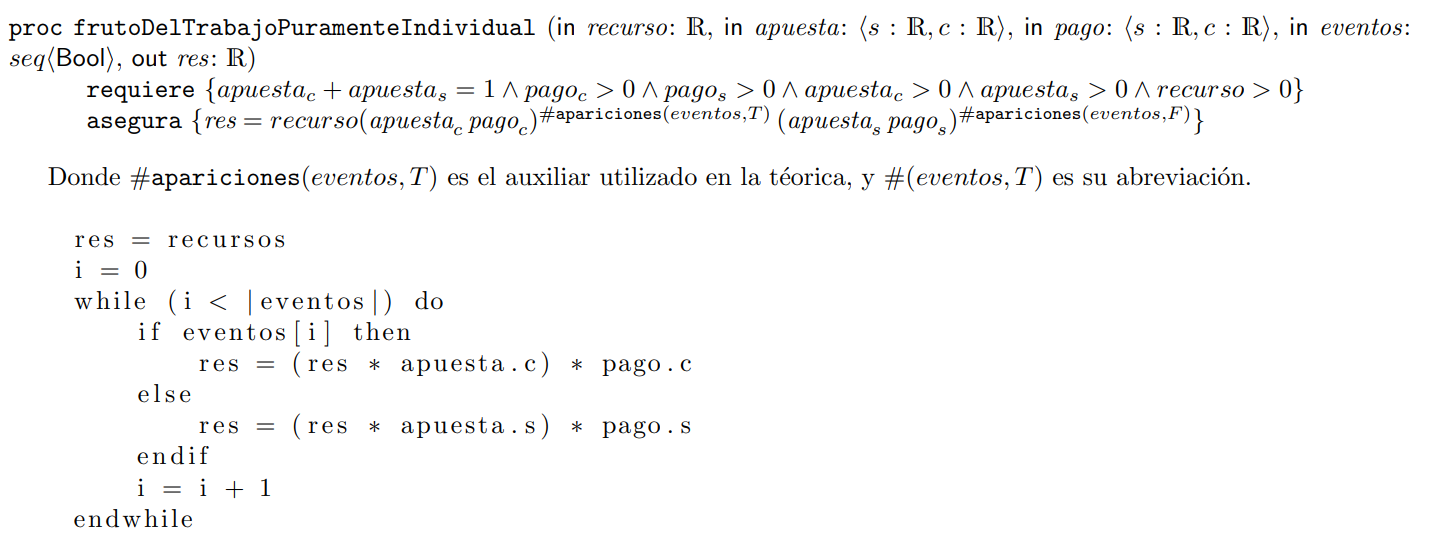
\includegraphics[width=0.9\textwidth]{codigo a resolver.png}
    \caption{\centering{Especificación a tratar con su implementación correspondiente}}
    \label{fig:codigo a resolver}
\end{figure}
Para demostrar que esta especificación es correcta respecto de su implementación vamos a definir la implementación como el programa $S$ y fragmentarlo de la siguiente manera:
\begin{itemize} \setlength\itemsep{0cm}
    \item{S_1 \equiv $\lbrace$
  	\begin{lstlisting}[label=code:s1]
res = recursos;
i = 0;
	\end{lstlisting} 
 }$\rbrace$
    \item{S_2 \equiv $\lbrace$
  	\begin{lstlisting}[label=code:s2]
if eventos[i] then
    res = (res * apuesta.c) * pago.c
else
    res = (res * apuesta.s) * pago.s
endif
i = i + 1
	\end{lstlisting} 
     \item{S_3 \equiv $\lbrace$
  	\begin{lstlisting}[label=code:s]
while (i < |eventos|) do 
   S2;
endwhile
	\end{lstlisting} 
 }$\rbrace$
\end{itemize}\textbf{}
El programa será correcto si y solo si el predicado $Pre \implicaLuego wp(S, Post)$ es verdadero, con Pre y Post como la precoindición y postcondición de la especificación. Para corroborar esto primero demostraremos lo siguiente:
\begin{enumerate} \setlength\itemsep{0cm}
	\item $Pre\implicaLuego wp(S_1, P_c)$
    \item $P_c\implicaLuego wp(S_3, Post)$
\end{enumerate}
Donde $P_c \equiv \lbrace i=0 \land res = recursos\rbrace$\\\\
Habiendo probado lo listado anteriormente, podremos decir que como valen los puntos 1 y 2, por monotonía, el predicado $Pre \implicaLuego wp(S, Post)$ es verdadero y por consecuente que el programa es correcto
\clearpage
\subsection{$Pre\implicaLuego wp(S_1, P_c)$}
Para demostrar esta implicación debemos asumir que la precondición de la especificación es verdadera y a partir de ahí llegar a $wp(S_1, P_c)$ por lo cual primero debemos obtener $wp(S_1, P_c)$\\\\ 
$wp(S_1, p_c)\equiv wp(res = recursos; i = 0, \lbrace i=0 \land res = recursos\rbrace)$
\\\\ Por el axioma 1 sabemos que esto es equivalente a\\\\
$wp(res = recursos, wp(i = 0, \lbrace i=0 \land res = recursos\rbrace))$\\
Entonces vamos a obtener $wp(i = 0, \lbrace i=0 \land res = recursos\rbrace)$\\\\
$wp(i = 0, \lbrace i=0 \land res = recursos\rbrace) \equiv \lbrace res = recursos\rbrace \implies$ \\\\
$wp(res = recursos, wp(i = 0, \lbrace i=0 \land res = recursos\rbrace)) \equiv wp(res = recursos, \lbrace res = recursos\rbrace) \equiv true$ \\\\
Como $wp(S_1, P_c) \equiv true$ puedo confirmar que $Pre \implicaLuego wp(S_1, P_c)$ es verdadero.

\subsection{$P_c\implicaLuego wp(S_3, Post)$}
El programa $S_3$ al ser un ciclo, para poder demostrar esta implicación debemos utilizar el teorema de corrección de ciclo el cual marca que la tripla de Hoare 
\\\\ $\lbrace$$P_{c}$$\rbrace$
  	\begin{lstlisting}[label=code:s]
while (B) do 
   S2;
endwhile
	\end{lstlisting} 
$\lbrace$$Q_{c}$$\rbrace$\\\\
$\equiv P_c\implicaLuego wp(S_3, Post)$ \\\\
Es verdadera si, dado un predicado I, se cumplen las siguientes condiciones:

\begin{enumerate} \setlength\itemsep{0cm}
	\item $P_{c}\implies{I}$
	\item $\lbrace I\land B\rbrace S_2\lbrace I\rbrace$
	\item $I \land \lnot B \implies Q_c$
    \item $\lbrace I \land B \land v_0=fv\rbrace S_2 \lbrace fv<v_0\rbrace$
    \item $I \land fv \leq 0 \implies \lnot B$
\end{enumerate}

Siendo

\begin{itemize}
  \item $I=\lbrace0\leq i \leq |eventos| \yLuego \\ res = recursos {(apuestas_c*pago_c)}^{#apariciones(subseq(eventos,0,i),T)}*{(apuestas_s*pago_s)}^{#apariciones(subseq(eventos,0,i),F)}\rbrace$
  \item $B=\lbrace i<|eventos|\rbrace$
  \item $Q_c=Post$
  \item $fv=|eventos| - i$
\end{itemize}
\clearpage
A partir del invariante propuesto I se quieren probar las condiciones del teorema:

\begin{enumerate} \setlength\itemsep{0cm}
	\item $P_{c}\implies{I}$\\ \\ $\lbrace i=0 \land res = recursos\rbrace \implies \lbrace0\leq i \leq |eventos| \yLuego \\ res = recursos {(apuestas_c*pago_c)}^{#apariciones(subseq(eventos,0,i),T)}*{(apuestas_c*pago_c)}^{#apariciones(subseq(eventos,0,i),F)}\rbrace$\\ \\
 utilizando que i=0 y que la función subseq(eventos,0,i=0) = $\langle \rangle$ \\\\$\lbrace i=0 \land res = recursos\rbrace \implies \lbrace0\leq i \leq |eventos| \yLuego \\  res = recursos {(apuestas_c*pago_c)}^{#apariciones(\langle \rangle,T)}*{(apuestas_c*pago_c)}^{#apariciones(\langle \rangle,F)} \rbrace$ \\\\ utilizando que $#apariciones(\langle \rangle,T )=#apariciones(\langle \rangle,F )=0 $ \\\\ $\lbrace i=0 \land res = recursos\rbrace \implies \lbrace0\leq i \leq |eventos| \yLuego res = recursos*{(apuestas_c*pago_c)}^{0}*{(apuestas_c*pago_c)}^{0}=recursos \rbrace$\\\\ lo cual es cierto dado que si $i=0 \implies 0 \leq 0 \leq |eventos|$  y res=recursos $\implies$ res=recursos 
 \\

 
    
	\item $\lbrace I\land B\rbrace S_2\lbrace I\rbrace$ \\\\
  $B=\lbrace i<|eventos|\rbrace$ \\ $I=\lbrace0\leq i \leq |eventos| \yLuego \\ res = recursos {(apuestas_c*pago_c)}^{#apariciones(subseq(eventos,0,i),T)}*{(apuestas_c*pago_c)}^{#apariciones(subseq(eventos,0,i),F)}\rbrace$ \\ $I\land B = \lbrace0\leq i < |eventos| \yLuego \\ res = recursos {(apuestas_c*pago_c)}^{#apariciones(subseq(eventos,0,i),T)}*{(apuestas_c*pago_c)}^{#apariciones(subseq(eventos,0,i),F)}$
 
 \\\\ para probar esto, se utiliza el teorema que dice que $\lbrace P \rbrace S \lbrace Q \rbrace $ es valida sii  $\lbrace P \rbrace \implies wp(S,P) $, lo cual en este problema sería:\\\\ $\lbrace I\land B\rbrace \implies wp(S,I) $ \\\\ $\lbrace i<|eventos| \land 0\leq i \leq |eventos| \yLuego \\ res = recursos {(apuestas_c*pago_c)}^{#apariciones(subseq(eventos,0,i),T)}*{(apuestas_c*pago_c)}^{#apariciones(subseq(eventos,0,i),F)}\rbrace \\ \implies wp(S,I)\\\\ \lbrace 0\leq i < |eventos| \yLuego \\ res = recursos {(apuestas_c*pago_c)}^{#apariciones(subseq(eventos,0,i),T)}*{(apuestas_c*pago_c)}^{#apariciones(subseq(eventos,0,i),F)}\rbrace \\ \implies wp(S,I)$ \\\\Definimos res como oldres, por lo tanto queremos ver que Wp(S,I) cumple : \\\\ $Wp(S,I)=Wp(\IfThenElse{ev[i]=True}{res=(oldres*A_c)P_c}{res=(oldres*A_s)P_s};i:=i+1,I)$ \\\\ $Wp(S,I)=Wp(\IfThenElse{ev[i]=True}{res=(oldres*A_c)P_c}{res=(oldres*A_s)P_s},{I}^{i}_{i+1})=$\\\\$def(ev[i]) \yLuego ((ev[i] = True \land wp(res=(oldres*A_c)P_c,{I}^{i}_{i+1})) \lor (\lnot ev[i] =True\land wp(res=(oldres*A_s)P_s,{I}^{i}_{i+1}))) $ \\\\ 

 Utilizando $def(ev[i]) = 0 \leq i < |eventos|$ se simplifica $(0 \leq i < |eventos| \land 0 \leq i+1 \leq |eventos| )= 1 \leq i+1 \leq |eventos|$ y  wp(S,I) queda: \\\\ $Wp(S,I)= 0 \leq i < |eventos| \land ((ev[i] = True \land wp(res=(oldres*A_c)P_c,{I}^{i}_{i+1})) \lor (\lnot ev[i] =True\land wp(res=(oldres*A_s)P_s,{I}^{i}_{i+1})))\\\\Wp(S,I)= 0 \leq i < |eventos| \land ((ev[i] = True \land {({I}^{i}_{i+1})}^{res}_{(oldres*A_c)*P_c})) \lor (\lnot ev[i] =True\land {{I}^{i}_{i+1}}^{res}_{(oldres*A_s)*P_s}))\\\\Wp(S,I)= 0 \leq i < |eventos| \land ((ev[i] = True \yLuego 0\leq i+1 \leq |eventos| \yLuego \\   (oldres*A_c)P_c  = recursos {(apuestas_c*pago_c)}^{#apariciones(subseq(eventos,0,i+1),T)}*\\{(apuestas_s*pago_s)}^{#apariciones(subseq(eventos,0,i+1),F)}) \lor (\lnot ev[i] = True \yLuego 0\leq i+1 \leq |eventos| \yLuego \\ (oldres*A_s)P_s = recursos {(apuestas_c*pago_c)}^{#apariciones(subseq(eventos,0,i+1),T)}*\\{(apuestas_s*pago_s)}^{#apariciones(subseq(eventos,0,i+1),F)})) $ \\\\   Para simplificar veamos que:\\\\ $recursos {(apuestas_c*pago_c)}^{#apariciones(subseq(eventos,0,i+1),T)}*{(apuestas_s*pago_s)}^{#apariciones(subseq(eventos,0,i+1),F)}$ \ $ =recursos {(apuestas_c*pago_c)}^{#apariciones(subseq(eventos,0,i),T)}*{(apuestas_c*pago_c)}^{#apariciones(subseq(eventos,i,i+1),T)}*{(apuestas_s*pago_s)}^{#apariciones(subseq(eventos,0,i),F)}*{(apuestas_s*pago_s)}^{#apariciones(subseq(eventos,i,i+1),F)} $ \ $ =oldres*{(apuestas_c*pago_c)}^{#apariciones(subseq(eventos,i,i+1),T)}*{(apuestas_s*pago_s)}^{#apariciones(subseq(eventos,i,i+1),F)}$ \\
 
 por lo tanto: \\\\$Wp(S,I)= 0 \leq i < |eventos| \land ((ev[i] = True \land \\(oldres*A_c)P_c=oldres*{(apuestas_c*pago_c)}^{#apariciones(subseq(eventos,i,i+1),T)}*\\{(apuestas_s*pago_s)}^{#apariciones(subseq(eventos,i,i+1),F)}) \lor \\(\lnot ev[i] =True\land (oldres*A_s)P_s = oldres*{(apuestas_c*pago_c)}^{#apariciones(subseq(eventos,i,i+1),T)}*\\{(apuestas_s*pago_s)}^{#apariciones(subseq(eventos,i,i+1),F)}$\\\\ Lo cual nos dice que en caso de que ev[i]=True sea cierto entonces apariciones(subseq(eventos,i,i+1),T)=1 y se cumpliría $(oldres*A_c)P_c=oldres*{(apuestas_c*pago_c)}^{1}*{(apuestas_s*pago_s)}^{0}$, en caso contrario se cumpliría $(oldres*A_s)P_s=oldres*{(apuestas_c*pago_c)}^{0}*{(apuestas_s*pago_s)}^{1}$
 
 
	\item $I \land \lnot B \implies Q_c$ \\\\ $I=\lbrace0\leq i \leq |eventos| \yLuego \\ res = recursos {(apuestas_c*pago_c)}^{#apariciones(subseq(eventos,0,i),T)}*{(apuestas_s*pago_s)}^{#apariciones(subseq(eventos,0,i),F)}\rbrace,\\
 \lnot B=\lbrace i \geq |eventos|\rbrace\\ Q_c=\lbrace res = {recursos * (apuesta.c * pago.c)}^{\#apariciones(eventos, True)}*(apuesta.s * pago.s)^{\#apariciones(eventos, False)}\rbrace\\\\ $Utilizando que $ 
 I \land \lnot B\implies 0\leq i\leq |eventos| \land i\geq|eventos| \implies i=|eventos|\\
 i=|eventos| \implies subseq(eventos, 0, i) = eventos\\\\ $podemos reducir $I \land \lnot B$ a \\\\$ I \land \lnot B = \lbrace i=|eventos| \land res = recursos {(apuestas_c*pago_c)}^{#apariciones(eventos,T)}$\\$*{(apuestas_s*pago_s)}^{#apariciones(eventos,F)} \equiv Q_c \rbrace
 $ \\\\ lo cual sería equivalente a \\\\ $i=|eventos| \land Q_c \implies Q_c$ \\\\ que es lo que queriamos probar.
  
    
    \clearpage
    \item $\lbrace I \land B \land v_0=f_v\rbrace S_2 \lbrace fv<v_0\rbrace$\\\\
    $fv=|eventos| - i$\\
    $v_o=f_v$ 
    $I=\lbrace0\leq i \leq |eventos| \yLuego \\ res = recursos {(apuestas_c*pago_c)}^{#apariciones(subseq(eventos,0,i),T)}*{(apuestas_s*pago_s)}^{#apariciones(subseq(eventos,0,i),F)}\rbrace $
    $B=\lbrace i<|eventos|\rbrace$\\ $(I\land B \land v_o=f_v)= \lbrace0\leq i < |eventos| \yLuego \\ res = recursos {(apuestas_c*pago_c)}^{#apariciones(subseq(eventos,0,i),T)}*{(apuestas_c*pago_c)}^{#apariciones(subseq(eventos,0,i),F)} \land f_v= |eventos| - i \land v_o= f_v$

    Esto es equivalente a demostrar que $\lbrace I \land B \land v_0=fv \rbrace \implies wp(S,f_v < v_o)$ veamos como queda la wp :\\\\$
    wp(if .... endif; i:= i+1,|eventos| - i < v_o)\\wp(if .... endif,wp(i:= i+1,|eventos| - i < v_o))\\wp(if...endif,{{(|eventos| - i)}^{i}}_{i+1}< v_o)\\\\(eventos[i]=True \land wp(res=(res*apuesta.c)*pago.c,|eventos| - (i+1)< v_o)) \lor (eventos[i]=False \land wp(res=(res*apuesta.s)*pago.s,|eventos| - (i+1)< v_o))\\ \\(eventos[i]=True \land {{(|eventos| - (i+1))}^{res}}_{(res*apuesta.c)*pago.c}< v_o) \lor \\(eventos[i]=False \land {{(|eventos| - (i+1))}^{res}}_{(res*apuesta.s)*pago.s}< v_o)\\\\ (eventos[i]=True \land (|eventos| - (i+1))< v_o) \lor (eventos[i]=False \land (|eventos| - (i+1))< v_o)\\\\ (eventos[i]=True \lor eventos[i]=False) \land (|eventos| - (i+1))< v_o \\\\ (|eventos| - (i+1))< v_o$ \\\\Como $f_v = v_0$ equivale a |eventos| - i, reemplazamos $v_0$ con esa expresión:\\\\$(|eventos| - (i+1))<|eventos| - i\\- (i+1)< - i\\ i+1 > i$\\Lo cual es verdadero. Por lo tanto, demostramos que:\\ $\lbrace I \land B \land v_0=fv\rbrace \implies wp(S,f_v < v_o)$
    
    
    
    \item $I \land fv \leq 0 \implies \lnot B$ \\\\ $fv=|eventos| - i \leq 0 \implies  |eventos| \leq i \\ I=\lbrace0\leq i \leq |eventos| \yLuego \\ res = recursos {(apuestas_c*pago_c)}^{#apariciones(subseq(eventos,0,i),T)}*{(apuestas_c*pago_c)}^{#apariciones(subseq(eventos,0,i),F)}\rbrace \\ 
 \lnot B=\lbrace i \geq |eventos|\rbrace$\\ Utilizando $|eventos| \leq i \land 0\leq i \leq |eventos| \implies \lbrace i=|eventos| \rbrace $ se obtiene :\\\\ $ \lbrace i =|eventos| \yLuego \\ res = recursos {(apuestas_c*pago_c)}^{#apariciones(subseq(eventos,0,i),T)}*{(apuestas_s*pago_s)}^{#apariciones(subseq(eventos,0,i),F)} \rbrace \\ \implies  \lbrace i \geq |eventos| \rbrace$ \\\\ Lo cual es cierto dado que  $\lbrace i=|eventos| \rbrace \implies  \lbrace i \geq |eventos| \rbrace $ 

 
\end{enumerate}
\subsection{Conclusión}
Como dijimos previamente, habiendo demostrado que valen los puntos 1 y 2 el predicado $Pre \implicaLuego wp(S, Post)$ es verdadero por monotonía y por lo tanto programa es correcto
\clearpage
\section{Anexo}

\begin{figure}[H]
    \centering
    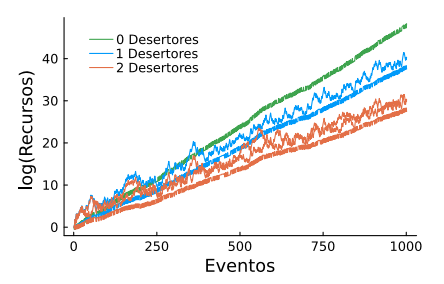
\includegraphics[width=0.45\textwidth]{Estudio apuestas.png}
    \caption{\centering{Recursos resultantes a lo largo de los eventos para 100 participantes, en verde se ve el caso donde todos los participantes aportan al fondo comun, en azul y rojo los casos con 1 y 2 desertores .}}
    \label{fig:modelo apuestas}
\end{figure}

En la \autoref{fig:modelo apuestas} se ven los resultados obtenidos en un trabajo, donde se obtiene que  al aumentar la cantidad de desertores, a pesar de que estos obtienen mejores resultados que el grupo participante del fondo común, los recursos para desertores y contribuyentes son inferiores a largo plazo que si todos hubiesen contribuido al fondo común. En caso de implementar un algoritmo como el tratado en este trabajo se buscaría obtener resultados consistentes con estos. 
\newpage
\printbibliography

\end{document}


